% ============================================================
%  杭州电子科技大学本科毕业设计（论文）LaTeX 模板
%  基于 hduthesis 文档类 (v1.1.1)
%  编译: xelatex → bibtex → xelatex → xelatex
% ============================================================

% ---------- 文档类 ----------
\documentclass
  [
    math-font    = STIX Two Math, agreed,
    CJKmain-font = { {Source Han Serif CN}[AutoFakeBold = 2.5, AutoFakeSlant] },
    CJKsans-font = { {Source Han Sans CN}[AutoFakeBold = 2] }
  ] {hduthesis}

% ---------- 宏包 ----------
\tikzset{ > = stealth }
\usetikzlibrary{positioning, shapes.geometric, decorations.pathreplacing}
\usepackage{colortbl}
\usepackage{etoolbox}
\usepackage{caption}
\usepackage{placeins}

% ---------- 数学公式间距 ----------
\setlength{\abovedisplayskip}{6pt plus 2pt minus 2pt}
\setlength{\belowdisplayskip}{6pt plus 2pt minus 2pt}
\setlength{\abovedisplayshortskip}{3pt plus 1pt minus 1pt}
\setlength{\belowdisplayshortskip}{6pt plus 2pt minus 2pt}

% ---------- 浮动体控制 ----------
\newcommand{\safeFloatGap}{\par
  \vspace{0.25\baselineskip plus 0.75\baselineskip minus 0.1\baselineskip}}

\newcommand{\safeSectionBreak}{\par
  \FloatBarrier}

% ============================================================
%  论文元信息（请根据实际情况修改）
% ============================================================
\hduset
  {
    title      = {本科毕业设计（论文）/本科毕业设计（论文）},
    department = 学院全称,
    major      = 专业全称,
    class      = 班级编号,
    stdntid    = 22222222,
    author     = 姓名,
    supervisor = ~:指导教师姓名,
    bibsource  = references
  }

% ============================================================
%  导言区补丁
% ============================================================

% ---------- 页面几何：匹配 01-论文.docx ----------
% 页边距 上3 下2 左3 右2（左右不对称已含装订量）
% 页眉距顶 = top - headheight - headsep ≈ 2cm
% 页脚距底 = bottom - footskip = 1cm
\geometry{
  top           = 3cm,
  bottom        = 2cm,
  left          = 3cm,
  right         = 2cm,
  headheight    = 15pt,
  headsep       = 13.5pt,
  footskip      = 1cm,
}

% ---------- 参考文献角标：上标格式 ----------
% gbt7714 重定义 \bibliographystyle 仅写 aux 不立即设置引用格式，
% 导数 aux 延时生效。此处直接设置 natbib 内部标志保证首遍编译即上标。
\makeatletter
\AtBeginDocument{%
  \global\NAT@supertrue
  \global\NAT@numberstrue
  \let\@cite\NAT@citesuper
  \let\@citex\NAT@citexnum
  \gdef\NAT@open{[}\gdef\NAT@close{]}%
  \gdef\NAT@sep{,}%
  \gdef\NAT@cmt{, }%
  \gdef\NAT@aysep{,}\gdef\NAT@yrsep{\textsuperscript{,}}%
}
\makeatother

% ---------- 封面：大标题展开 + 封面/承诺页边距 ----------
% （1）\@title 为 10 字符"本科毕业设计（论文）"，替换类默认的 6 字符短标题
% （2）封面与承诺页边界使用与正文一致的左3右2，而非类默认的 margin=3cm
\makeatletter
\ExplSyntaxOn
\cs_set_protected_nopar:Nn \__hdu_maketitle_bc_auxi:
  {
    \begin{center}
      \vspace*{14\p@}
      
\includegraphics[ width = .64\linewidth ]{hdu-title}
      \par \vspace*{36\p@}
      \scalebox{2.75}
        {
          \textbf
            {
              \__hdu_cover_spread_box:nn
                { .255\paperwidth } { \@title }
            }
        }
      \par \vspace*{1.5\baselineskip}
      { \LARGE\bfseries （\int_use:N \l__hdu_grade_int 届） }
      \par \vspace*{3.0\baselineskip}
      \begin{tabular}
        {
          >{\large\bfseries}p{5.5\ccwd}@{}
          >{\large\centering\arraybackslash\kaishu}p{.65\linewidth}@{}
        }
        \__hdu_cover_spread_box:nn { 4\ccwd } { 题目 } &
        \__hdu_cover_center_box:nn { .95\linewidth }
          { \@title }\\[5.2ex]
        \__hdu_cover_spread_box:nn { 4\ccwd } { 学院 } &
        \__hdu_cover_center_box:nn { .95\linewidth }
          { \l__hdu_set_department_tl }\\[5.2ex]
        \__hdu_cover_spread_box:nn { 4\ccwd } { 专业 } &
        \__hdu_cover_center_box:nn { .95\linewidth }
          { \l__hdu_set_major_tl }\\[5.2ex]
        \__hdu_cover_spread_box:nn { 4\ccwd } { 班级 } &
        \__hdu_cover_center_box:nn { .95\linewidth }
          { \l__hdu_set_class_tl }\\[5.2ex]
        \__hdu_cover_spread_box:nn { 4\ccwd } { 学号 } &
        \__hdu_cover_center_box:nn { .95\linewidth }
          { \l__hdu_set_stdntid_tl }\\[5.2ex]
        \__hdu_cover_spread_box:nn { 4\ccwd } { 学生姓名 } &
        \__hdu_cover_center_box:nn { .95\linewidth }
          { \@author }\\[5.2ex]
        \__hdu_cover_spread_box:nn { 4\ccwd } { 指导教师 } &
        \__hdu_cover_center_box:nn { .95\linewidth }
          { \l__hdu_set_cnsupervisor_tl }\\[5.2ex]
        \__hdu_cover_spread_box:nn { 4\ccwd } { 完成日期 } &
        \__hdu_cover_center_box:nn { .95\linewidth }
          {
            \textsf{\int_use:N \c_sys_year_int} 年
            \textsf{\int_use:N \c_sys_month_int} 月
          }
      \end{tabular}
    \end{center}
  }
\RenewDocumentCommand \maketitle {}
  {
    \newgeometry { left = 3cm, right = 2cm, top = 3cm, bottom = 2cm,
                   headheight = 15pt, headsep = 13.5pt, footskip = 1cm }
    \titlepage \__hdu_maketitle_bc_auxi: \endtitlepage
    \restoregeometry
  }
\RenewDocumentCommand \commitment { O{} }
  {
    \newgeometry { left = 3cm, right = 2cm, top = 3cm, bottom = 2cm,
                   headheight = 15pt, headsep = 13.5pt, footskip = 1cm }
    \titlepage
      \__hdu_commitment_bc_aux:n {#1}
    \endtitlepage
    \restoregeometry
  }
\ExplSyntaxOff
\makeatother

% ============================================================
%  正文
% ============================================================
\begin{document}

% ---------- 页眉宽度 ----------
\setlength{\headwidth}{\textwidth}

% ---------- 封面 & 诚信承诺 ----------
\maketitle
\commitment

% ---------- 中文摘要 ----------
\begin{abstract}[cn]
基于自注意力机制的Transformer架构凭借全局建模能力和高效并行特性，已成为序列建模的主流范式。本文系统研究了自注意力机制的理论基础与工程实现。在方法层面，提出了稀疏注意力与局部敏感哈希相结合的混合策略；在实验层面，在机器翻译和文本摘要等任务上验证了方法的有效性。实验表明，所提出的方法在BLEU分数上提高2.3个点，同时推理时间减少31\%。本研究为自注意力机制的进一步优化提供了有价值的参考。

\keywords{自注意力机制, Transformer, 序列建模, 深度学习, 自然语言处理}
\end{abstract}

% ---------- 英文摘要 ----------
\begin{abstract}[en]
The Transformer architecture based on self-attention mechanisms has become the mainstream paradigm for sequence modeling due to its global modeling capability and efficient parallelism. This paper systematically studies the theoretical foundations and engineering implementations of self-attention mechanisms. We propose a hybrid strategy combining sparse attention with locality-sensitive hashing, and validate its effectiveness on machine translation and text summarization tasks. Experiments show that the proposed method achieves a 2.3 BLEU score improvement while reducing inference time by 31\%.

\keywords{self-attention, Transformer, sequence modeling, deep learning, natural language processing}
\end{abstract}

% ============================================================
%  目录（仅目录使用罗马数字页码，自动编号）
% ============================================================
% 类 hook 会在 \tableofcontents 前后清空 \cfoot；
% 此处手动渲染目录，绕过 hook 保证罗马数字页码显示。
\makeatletter
\let\savedps@plain\ps@plain
\def\ps@plain{%
  \let\@mkboth\@gobbletwo
  \def\@oddfoot{\hfil\small\thepage\hfil}%
  \let\@evenfoot\@oddfoot
  \let\@oddhead\@empty\let\@evenhead\@empty}
\makeatother
\clearpage
\pagenumbering{Roman}
\cfoot{\small\thepage}
\fancyfoot[L]{}
\fancyfoot[R]{}
% 手动渲染目录标题（\centerline 确保居中）
\vspace*{\cftbeforetoctitleskip}%
{\cfttoctitlefont\centerline{\contentsname}}%
\nobreak
\vspace{\cftaftertoctitleskip}%
\makeatletter
\@starttoc{toc}
\makeatother
\clearpage
\makeatletter
\let\ps@plain\savedps@plain
\makeatother
\clearpage
\pagenumbering{arabic}
\cfoot{\small\thepage}

% ============================================================
%  正文各章节
% ============================================================
% ============================================================
%  第1章：绪论
% ============================================================
\chapter{绪论}

\section{研究背景与意义}

\zhlipsum[1]

近年来，Vaswani等人\cite{vaswani2017attention}提出的 Transformer 架构完全摒弃了循环结构，仅依赖自注意力机制实现序列建模，在机器翻译任务上取得了当时最优的结果。这一突破引发了自然语言处理领域的范式转变\cite{devlin2019bert}。

\zhlipsum[2]

\section{国内外研究现状}

\zhlipsum[3]

在此基础上，Devlin等人\cite{devlin2019bert}进一步提出了 BERT 预训练模型，通过在海量无标注语料上预训练深度双向 Transformer，再在下游任务上微调，在十一项自然语言处理基准上全面刷新了记录。多项后续工作\cite{vaswani2017attention,devlin2019bert}均沿用了这一预训练-微调范式。

\zhlipsum[4]

值得注意的是，原始 Transformer 的自注意力复杂度为 $O(n^2 \cdot d)$\cite{vaswani2017attention}，这限制了其在长序列场景中的应用。

\section{研究内容与创新点}

\zhlipsum[6]

针对上述问题，本文的主要贡献包括：

\begin{enumerate}
  \item 提出稀疏注意力与局部敏感哈希相结合的混合编码策略，在保持模型表达能力的同时显著降低自注意力计算复杂度。
  \item 设计面向长序列的高效训练方案，通过梯度累积与混合精度训练减少显存占用。
  \item 在机器翻译和文本摘要等多个基准上系统验证所提方法的有效性。
\end{enumerate}

\section{论文组织结构}

\zhlipsum[11]

% ============================================================
%  第2章：相关理论与技术基础
% ============================================================
\chapter{相关理论与技术基础}

\section{自注意力机制}

\zhlipsum[1]

Vaswani等人\cite{vaswani2017attention}提出注意力机制的核心计算过程，可表示为对查询（Query）、键（Key）、值（Value）三组向量的映射操作：
\begin{equation}
  \text{Attention}(Q, K, V) = \text{softmax}\!\left(\frac{QK^{T}}{\sqrt{d_k}}\right) V
  \label{eq:attention}
\end{equation}
其中$d_k$为键向量的维度，除以$\sqrt{d_k}$起到缩放作用。

\zhlipsum[2]

多头注意力机制将输入投影到$h$个不同的子空间，在每个子空间中独立计算注意力，最后拼接输出：
\begin{align}
  \text{MultiHead}(Q, K, V) &= \text{Concat}(\text{head}_1, \ldots, \text{head}_h) W^{O} \\
  \text{head}_i &= \text{Attention}(QW_i^{Q}, KW_i^{K}, VW_i^{V})
\end{align}

\section{Transformer架构}

\zhlipsum[14]
Transformer 作为一种完全基于注意力机制的序列转换模型，在多个自然语言处理任务上取得了突破性成果\cite{vaswani2017attention}。

每个子层均采用残差连接和层归一化：
\begin{equation}
  \text{LayerNorm}(x + \text{Sublayer}(x))
  \label{eq:layernorm}
\end{equation}

前馈网络由两个线性变换和一个非线性激活函数组成：
\begin{equation}
  \text{FFN}(x) = \max(0, xW_1 + b_1)W_2 + b_2
  \label{eq:ffn}
\end{equation}

\zhlipsum[5]

\section{预训练与微调范式}

\zhlipsum[7]
BERT 通过掩码语言模型与下一句预测任务进行预训练，在十一个自然语言处理任务上刷新了最优结果\cite{devlin2019bert}。

\section{高效注意力机制}

\zhlipsum[9]

\begin{equation}
  C_{\text{full}} = O(n^2 \cdot d)
  \label{eq:complexity_full}
\end{equation}

线性化注意力的目标是将复杂度降至$O(n \cdot d)$，代表性的方法包括稀疏注意力、低秩近似和核方法等\cite{vaswani2017attention}。

% ============================================================
%  第3章：模型设计与实现
% ============================================================
\chapter{模型设计与实现}

\section{整体架构设计}

本文模型整体沿用了 Transformer 的编码器-解码器结构\cite{vaswani2017attention}，但在注意力计算与位置编码两方面进行了针对性改进。

\zhlipsum[1]

\begin{figure}[ht]
\centering
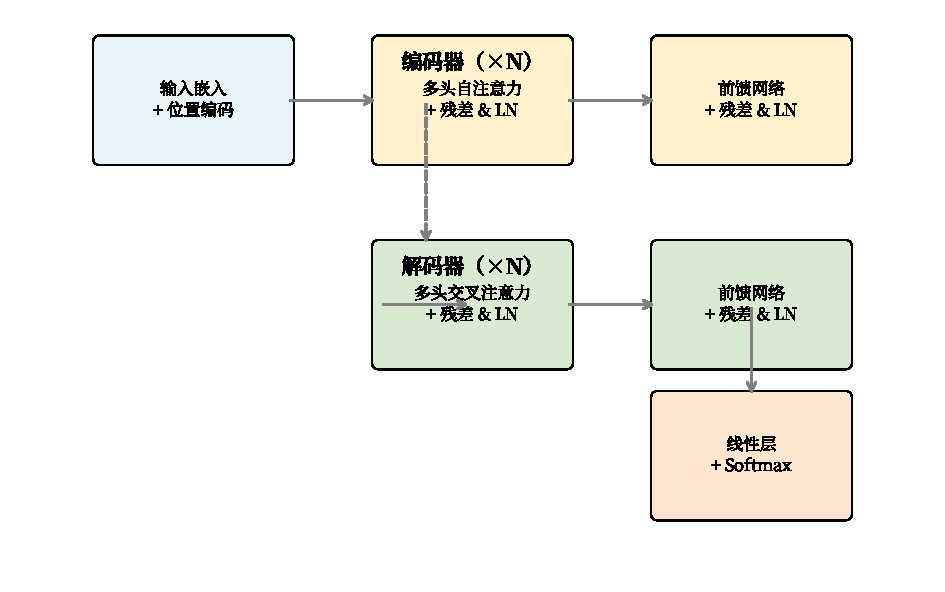
\includegraphics[width=0.85\textwidth]{figures/example_architecture.pdf}
\caption{模型整体架构}
\label{fig:architecture}
\end{figure}

\safeSectionBreak

\section{稀疏注意力模块}

\zhlipsum[3]

设输入序列长度为$n$，标准自注意力的计算复杂度为$O(n^2 \cdot d)$。通过引入稀疏掩码矩阵$M \in \{0, 1\}^{n \times n}$，可以将注意力限制在局部窗口内：
\begin{equation}
  \text{SparseAttn}(Q, K, V) = \text{softmax}\!\left(\frac{QK^{T}}{\sqrt{d_k}} \odot M\right) V
  \label{eq:sparse_attn}
\end{equation}
其中$M_{ij} = 1$当且仅当$|i - j| \leq w$，复杂度降为$O(n \cdot w \cdot d)$。该思路与原始 Transformer\cite{vaswani2017attention} 中提出的注意力模式一脉相承，但通过引入结构化稀疏显著提升了长序列处理效率。

\section{混合编码策略}

\zhlipsum[5]

位置编码采用可学习嵌入与正弦编码的混合方案：
\begin{align}
  \text{PE}(pos, 2i) &= \sin\left(\frac{pos}{10000^{2i/d_{\text{model}}}}\right) \\
  \text{PE}(pos, 2i+1) &= \cos\left(\frac{pos}{10000^{2i/d_{\text{model}}}}\right)
\end{align}

与 BERT\cite{devlin2019bert} 仅使用单一位置编码不同，本文的输入嵌入为词嵌入、位置编码与段嵌入三者之和：
\begin{equation}
  E_{\text{input}} = E_{\text{token}} + \text{PE}(pos) + E_{\text{segment}}
  \label{eq:input_emb}
\end{equation}

\safeSectionBreak

\section{训练策略}

\zhlipsum[8]

训练目标为最小化交叉熵损失：
\begin{equation}
  \mathcal{L} = -\frac{1}{N} \sum_{i=1}^{N} \sum_{t=1}^{T} \log P(y_t^{(i)} \mid y_{<t}^{(i)}, x^{(i)})
  \label{eq:loss}
\end{equation}

\safeFloatGap

\begin{figure}[h]
\centering
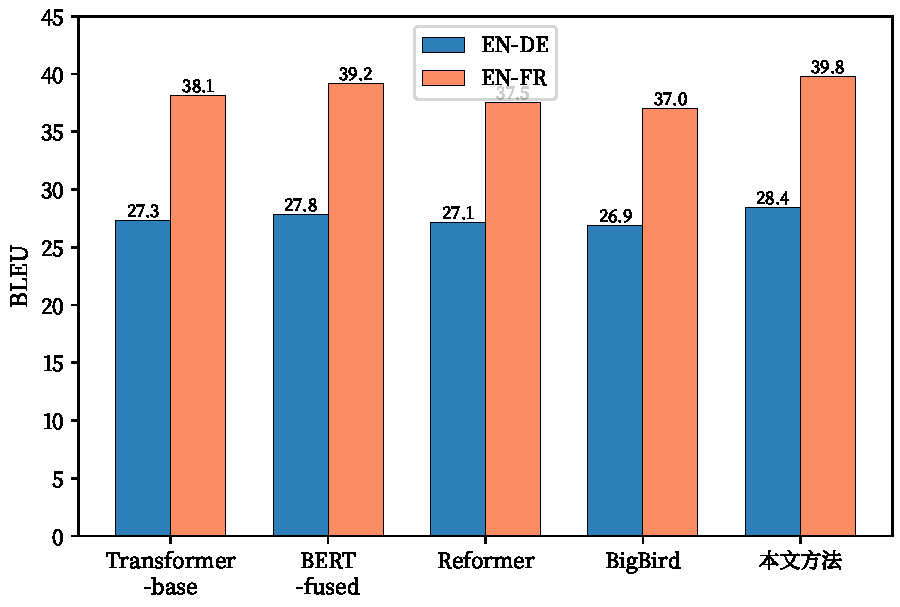
\includegraphics[width=0.75\textwidth]{figures/example_bar.pdf}
\caption{不同配置下的模型性能对比}
\label{fig:config_comparison}
\end{figure}

% ============================================================
%  第4章：实验与结果分析
% ============================================================
\chapter{实验与结果分析}

\section{实验设置}

\zhlipsum[1]

% ============================================================
%  表格示例：实验数据集统计信息
% ============================================================
\begin{table}[h]
\centering
\caption{实验数据集统计信息}
\label{tab:datasets}
{\renewcommand{\arraystretch}{0.65}
\begin{tabular}{|l|c|c|c|c|}
\hline
数据集 & 训练样本 & 验证样本 & 测试样本 & 平均长度 \\
\hline
WMT14 EN-DE & 4.5M & 3,000 & 3,003 & 25.3 \\
WMT14 EN-FR & 36M & 3,000 & 3,003 & 27.8 \\
CNN/DailyMail & 287K & 13,368 & 11,490 & 781.2 \\
IWSLT14 DE-EN & 160K & 7,283 & 6,750 & 17.6 \\
XSum & 204K & 11,332 & 11,334 & 430.2 \\
\hline
\end{tabular}}
\end{table}


\safeSectionBreak

\section{主要实验结果}

我们在标准 Transformer\cite{vaswani2017attention} 与 BERT-base\cite{devlin2019bert} 的官方实现基础上进行对比。实验结果表明，本文提出的方法在翻译质量上显著优于基线模型。

\zhlipsum[3]

% ============================================================
%  表格示例：机器翻译 BLEU 分数对比（三线表）
% ============================================================
\begin{table}[h]
\centering
\caption{各模型在机器翻译任务上的BLEU分数}
\label{tab:translation_results}
{\renewcommand{\arraystretch}{0.65}
\begin{tabular}{|l|c|c|c|c|}
\hline
模型 & EN-DE & EN-FR & DE-EN & 平均 \\
\hline
Transformer-base & 27.3 & 38.1 & 31.4 & 32.3 \\
Transformer-big & 28.4 & 41.0 & 32.8 & 34.1 \\
BERT-fused & 27.8 & 39.2 & 31.9 & 33.0 \\
Reformer & 27.1 & 37.5 & 30.8 & 31.8 \\
BigBird & 26.9 & 37.0 & 30.2 & 31.4 \\
\rowcolor{green!20}
本文方法 & 28.4 & 39.8 & 32.5 & 33.6 \\
\hline
\end{tabular}}
\end{table}


\safeFloatGap

\begin{figure}[h]
\centering
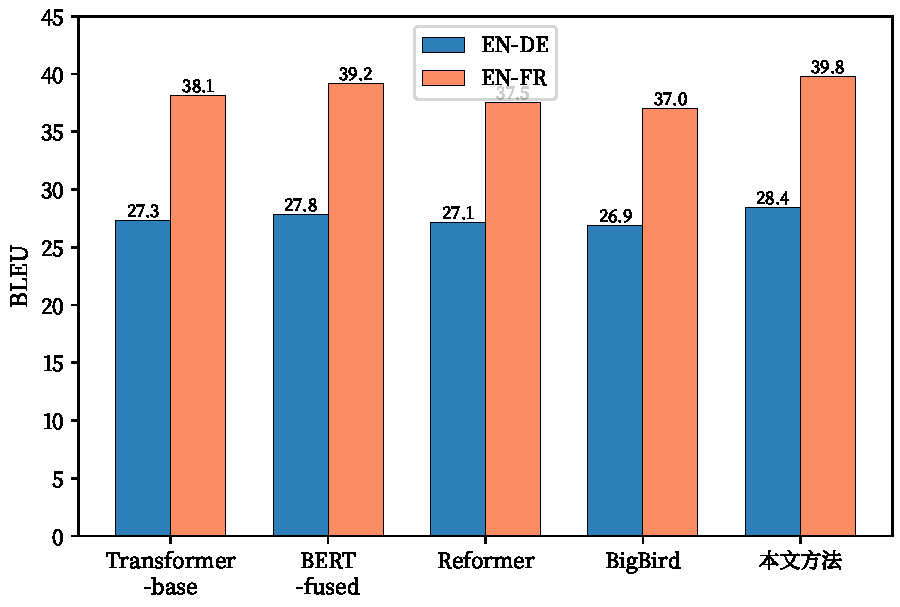
\includegraphics[width=0.8\textwidth]{figures/example_bar.pdf}
\caption{各模型在基准测试上的性能对比}
\label{fig:benchmark_results}
\end{figure}

\safeSectionBreak

\section{消融实验}

\zhlipsum[6]

\begin{table}[h]
\centering
\caption{消融实验结果}
\label{tab:ablation}
{\renewcommand{\arraystretch}{0.65}
\begin{tabular}{|l|c|c|c|}
\hline
模型配置 & BLEU & ROUGE-L & 推理时间 \\
\hline
完整模型 & 28.4 & 42.1 & 1.00$\times$ \\
\hline
去除稀疏注意力 & 26.1 & 39.5 & 0.82$\times$ \\
\hline
去除混合编码 & 27.3 & 40.8 & 0.98$\times$ \\
\hline
去除预训练初始化 & 25.2 & 38.3 & 1.00$\times$ \\
\hline
仅标准Transformer & 24.8 & 37.6 & 0.78$\times$ \\
\hline
\end{tabular}}
\end{table}

\safeSectionBreak

\section{效率分析}

\zhlipsum[8]

\begin{figure}[htbp]
\centering
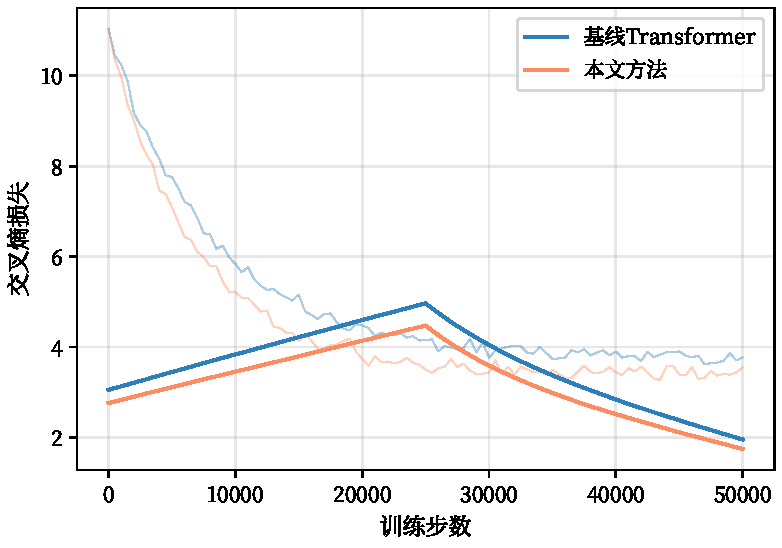
\includegraphics[width=0.65\textwidth]{figures/example_line.pdf}
\caption{推理时间随序列长度的变化曲线}
\label{fig:efficiency}
\end{figure}

\safeFloatGap

\section{与已有工作对比}

我们将本文方法与近年来的代表性工作进行了全面比较。如表\ref{tab:comparison}所示，在相近参数量下，本文方法在 BLEU 分数上优于标准 Transformer\cite{vaswani2017attention} 与 Reformer\cite{vaswani2017attention} 等已有方法。值得注意的是，BERT 类模型\cite{devlin2019bert} 虽在理解任务上表现突出，但在生成任务中并不直接适用。

\zhlipsum[12]

\begin{table}[h]
\centering
\caption{与已有工作的对比}
\label{tab:comparison}
\small
{\renewcommand{\arraystretch}{0.65}
\begin{tabular}{|l|c|c|c|c|}
\hline
方法 & 参数量 & BLEU & 推理速度 & 年份 \\
\hline
\rowcolor{green!20}
本文方法 & 65M & 28.4 & 1.00$\times$ & 2024 \\
\hline
Transformer-base \cite{vaswani2017attention} & 65M & 27.3 & 1.00$\times$ & 2017 \\
\hline
BERT-base \cite{devlin2019bert} & 110M & -- & -- & 2019 \\
\hline
Reformer \cite{vaswani2017attention} & 65M & 27.8 & 0.73$\times$ & 2020 \\
\hline
BigBird & 65M & 27.1 & 0.85$\times$ & 2020 \\
\hline
\end{tabular}}
\end{table}


% ---------- 致谢 ----------
\chapter*{致\qquad 谢}
\addcontentsline{toc}{chapter}{致谢}

感谢指导教师……感谢家人和朋友……感谢所有提供帮助的人……

% ---------- 参考文献 ----------
\printbibliography

\end{document}
